\documentclass[12pt]{article}
\textwidth=17cm \oddsidemargin=-0.9cm \evensidemargin=-0.9cm
\textheight=23.7cm \topmargin=-1.7cm
\headheight=14.5pt

\usepackage{amssymb, amsmath, amsfonts}
\usepackage{moreverb}
\usepackage{graphicx}
\usepackage{enumerate}
\usepackage{graphics}
\usepackage{color}
\usepackage{array}
\usepackage{float}
\usepackage{hyperref}
\usepackage{textcomp}
\usepackage{alltt}
\usepackage{physics}
\usepackage{mathtools}
\usepackage{tikz}
\usetikzlibrary{positioning}
\usetikzlibrary{arrows}
\usepackage{bigints}
\usepackage[utf8]{inputenc}
\usepackage[english]{babel}
\usepackage{amsthm}
\usepackage{fancyhdr}
\usepackage[makeroom]{cancel}
\pagestyle{fancy}
\allowdisplaybreaks

\newcommand{\E}{\varepsilon}

\newcommand{\suchthat}{\, \mid \,}
\newcommand{\ol}[1]{\overline{#1}}
\newcommand{\bbar}[1]{\overline{#1}}
\newcommand{\inpd}[1]{{\left< \, #1 \, \right>}}
\renewcommand{\theenumi}{\alph{enumi}}
\newcommand\Wider[2][3em]{%
\makebox[\linewidth][c]{%
  \begin{minipage}{\dimexpr\textwidth+#1\relax}
  \raggedright#2
  \end{minipage}%
  }%
}

\def\R{\mathbb{R}}
\def\C{\mathbb{C}}
\def\H{\mathcal{H}}
\DeclareMathOperator*{\esssup}{\text{ess~sup}}
\newcommand{\resolv}[1]{\rho(#1)}
\newcommand{\spec}[1]{\sigma(#1)}
\newcommand{\iffR}{\noindent \underline{$\Longrightarrow$:} }
\newcommand{\iffL}{\noindent \underline{$\Longleftarrow$:} }
\newcommand{\lightning}{\textbf{\Huge \Lightning}}
\newcommand{\spt}[1]{\text{spt}(#1)}
\def\ran{\text{ ran}}
   
\newenvironment{myprob}[1]
    {%before text commands
    %{\Huge \_ \_ \_ \_ \_ \_ \_ \_ \_ \_ \_ \_ \_ \_ \_ \_ \_ \_ } \\
    \noindent{\Huge$\ulcorner$}\textbf{#1.}\begin{em}
    }
    { 
    %after text commands
    \end{em} \\ \hphantom{l} \hfill {\Huge$\lrcorner$} }
%	{\noindent \rule{7.5cm}{2pt} \textgoth{#1} \rule{8.cm}{2pt} \begin{em}}
%	{\end{em}\\ \vspace{0.1pt}\noindent \rule{\textwidth}{2pt}}
%
\setcounter{section}{-1}




\begin{document}
\lhead{MATH228B}
\chead{Carter Johnson - Homework 03}
\rhead{\today}

{\let\newpage\relax} 


%%%%%%%%%%%%%%%%%%%%%%%%%%%%%%%%%%%%%%%%%%%%%%%%%%%%% P2
\begin{myprob}{Problem 1}
Consider 
$$u_t = 0.1 \Delta u \text{ on } \Omega = (0,1) \times (0,1) $$
$$\dfrac{\partial u}{\partial \vec{n}}=0 \text{ on } \delta \Omega $$
$$u(x,y,0)=\exp\qty(-10\qty((x-0.3)^2+(y-0.4)^2)) .$$
Write a program to solve this PDE using the Peaceman-Rachford ADI
scheme on a cell-centered grid. Use a direct solver for the tridiagonal
systems. In a cell-centered discretization the solution is stored at the
grid points $(x_i,y_j)=\qty(\Delta x(i-0.5),\Delta x(j-0.5))$ for $i,j = 1, \dots, N$ and $\Delta x = 1/N$. 
\end{myprob}
\begin{enumerate}[(a)]
\item Perform a refinement study to show that your numerical solution is second-order accurate in space and time (refine time and space simultaneously using $\Delta t = \Delta x$) at time $t=1$.

The one-dimensional discrete Laplacian for homogeneous Neumann boundary conditions is 
$$L = \dfrac{1}{\Delta x^2}\qty(\begin{array}{cccccc}
-1 & 1 &  & & \\
1 & -2 & 1 &  & \\
& \ddots & \ddots & \ddots & \\
& & 1 & -2 & 1 \\
& & & 1 & -1 \\
\end{array}).$$
Using this matrix for both $L_x$ and $L_y$ (since $\Delta x = \Delta y$), I implemented the Peaceman-Rachford ADI scheme
\begin{align*}
\qty(I - \dfrac{0.1 \Delta t}{2} L)u^* &= \qty(I + \dfrac{0.1 \Delta t}{2}L)u^n \\
\qty(I - \dfrac{0.1 \Delta t}{2} L)u^{n+1} &= \qty(I + \dfrac{0.1 \Delta t}{2}L)u^*.
\end{align*}
Using $\Delta t = \Delta x$, I performed a refinement study on the scheme for $\Delta x = 2^{-1}, \dots, 2^{-9}$.  Since the analytic solution is not known, I used successive differences to demonstrate the second-order accuracy. The successive differences were computed by comparing the numerical solution $u^{(i)}(x,y,1)$ for $\Delta x = 2^{-i}$ with a simple coarsening of the solution $u^{(i+1)}(x,y,1)$ for $\Delta x = 2^{-(i+1)}$ in the discrete 1-norm
$$d_{i+1} = (2^{-i})^2 \norm{\text{restrict}(u^{(i+1)}) - u^{(i)}}_1, $$
where $\norm{\cdot}_1$ is the matrix one-norm (max(sum(abs(x), axis=0))).
The successive differences and the ratios between them are given in Table 1.  The table shows that as we reduce the grid/time spacing by a factor of 2, the successive differences are reduced by a factor of 4, hence the scheme is indeed second-order accurate in time and space.

\begin{table}[H]
\caption{Peaceman-Rachford ADI Successive Differences and Ratios}
\centering\begin{tabular}{||c|cc||}
\hline \hline
   $\Delta x = \Delta t$ &  $d_i$ &   $d_{i-1}/d_{i}$ \\
\hline \hline
                $2^{-1}$      &            ------       &        ------   \\
                $2^{-2}$    &              0.00550621  &       ------   \\
                $2^{-3}$    &      0.00236241  &             2.33076  \\
                $2^{-4}$     &         0.000234787 &            10.0619\\
                $2^{-5}$      &       5.57923e-05 &             4.20823 \\
                $2^{-6}$       &       1.38646e-05 &             4.02407  \\
                $2^{-7}$        &      3.45834e-06 &             4.00904  \\
                $2^{-8}$         &    8.63688e-07 &             4.00416 \\
                $2^{-9}$          &    2.15822e-07 &             4.00184 \\
                $2^{-10}$          &     5.39421e-08 &             4.001 \\
\hline \hline
\end{tabular}
\end{table}


\item Time your code for different grid sizes. Show how the computational time scales with the grid size. Compare your timing results with those from the previous homework assignment for Crank-Nicolson.

Table 2 shows that PR-ADI vastly outperforms my Crank-Nicolson code from last assignment.  However, PR-ADI had no visible runtime scaling, much like CN last homework, but it may be climbing up to a scaling factor of 16 asymptotically.  As we reduce the grid and time spacing by a factor of 2, we should increase the total runtime by a factor of 16.  This is the same scaling than in Crank-Nicolson.  In PR-ADI, we're inverting $N\times N$-size, tridiagonal matrices as opposed to CN, which inverts $N^2\times N^2$-size, banded matrices.  The work to invert an $N\times N$ tridiagonal matrix is only $\mathcal{O}(N)$, but we have to invert $N$ matrices of this size, so the work per timestep for PR-ADI is still $\mathcal{O}(N^2)$.  Since we use $\Delta t = \Delta x,$ we perform $N$ time steps, so the total work is $\mathcal{O}(N^3)$.  Hence, the runtimes \emph{should} increase by 8 when $\Delta x$ is reduced by a factor of 2.

\begin{table}[H]
\caption{PR-ADI vs. Crank-Nicolson Runtime Comparison}
\centering\begin{tabular}{||c|cc|cc||}
\hline \hline
   $\Delta x = \Delta t$ &   PR-ADI Runtimes $T$ &   $T_{i}/T_{i-1}$ &  CN Runtimes $T$ &   $T_{i}/T_{i-1}$ \\
\hline \hline
 $2^{-1}$        &   0.062193 &    -----       &       0.134055 &           --------   \\
                $2^{-2}$        &   0.00985  &         0.158378   &  0.136421 &            1.01765 \\
                $2^{-3}$       &   0.020712 &         2.10274 &    0.102737 &            0.753088 \\
                $2^{-4}$       &   0.045364 &         2.19023  &   0.151887 &            1.47841 \\
                $2^{-5}$      &   0.087029 &         1.91846  &  0.335359 &            2.20795    \\
                $2^{-6}$     &   0.192444 &         2.21126  &      2.63749  &            7.86469   \\
                $2^{-7}$    &   0.49876  &         2.59171  &    14.1191   &            5.35322   \\
                $2^{-8}$   &    2.7783   &         5.57042  &  93.7666   &            6.64112   \\
                $2^{-9}$   &  23.3481   &         8.40372   &   610.232    &            6.50799  \\
                $2^{-10}$  & 368.058    &        15.7639  &  -------- & ------ \\
\hline \hline
\end{tabular}
\end{table}

\item Show that the spatial integral of the solution to the PDE does not change in time. That is $$\dfrac{\dd }{\dd t} \int_\Omega u \ \dd V = 0.$$

\begin{align*}
\dfrac{\dd }{\dd t} \int_\Omega u \ \dd V &= \int_\Omega u_t \ \dd V &\text{by Lebesgue DCT} \\
&= 0.1 \int_\Omega \Delta u \ \dd V &\text{ by the PDE} \\
&= 0.1 \int_\Omega \grad \cdot (\grad u) \ \dd V &\text{by definition of $\Delta$} \\
&= 0.1 \int_{\delta \Omega} \grad u \cdot \vec{n} \ \dd s &\text{by Flux-Divergence Thm} \\
&= 0 &\text{ since $\dfrac{\partial u}{\partial \vec{n}}=0 \text{ on } \delta \Omega$. }
\end{align*}

\item  Show that the solution to the discrete equations satisfies the discrete conservation property
$$\sum_{i,j} u_{i,j}^n = \sum_{i,j} u^0_{i,j} $$
for all $n$. Demonstrate this property with your code.

Table 3 shows that the difference between the sums of the initial condition and every time step is close to machine precision, so the discrete conservation property holds.
\begin{table}[H]
\caption{Peaceman-Rachford ADI Scheme - Discrete Conservation Property, $\Delta x = 2^{-8}$, $\Delta t = 2^{-4}$.}
\centering\begin{tabular}{|cc|}
\hline \hline
Time Step $n$ ($n\Delta t$) & $\sum_{i,j} u_{i,j}^0 - \sum_{i,j} u^n_{i,j}$ \\
\hline  
1 & 5.82076609135e-11 \\
2 & 1.52795109898e-10 \\
3 & 2.11002770811e-10 \\
4 & 2.51020537689e-10 \\
5 & 2.65572452918e-10 \\
6 & 2.76486389339e-10 \\
7 & 2.83762346953e-10 \\
8 & 2.98314262182e-10 \\
9 & 3.16504156217e-10 \\
10 & 3.3833202906e-10 \\
11 & 3.56521923095e-10 \\
12 & 3.89263732359e-10 \\
13 & 4.14729584008e-10 \\
14 & 4.40195435658e-10 \\
15 & 4.69299266115e-10 \\
16 & 5.16592990607e-10 \\
\hline \hline
\end{tabular}
\end{table}

Table 4 shows the difference in the sums between the initial condition and the final solution $u(x,y,1)$ for various grid and time spacings.  The differences are close to machine precision, so the discrete conservation property holds.
\begin{table}[H]
\caption{Peaceman-Rachford ADI Scheme - Final Discrete Conservation Property}
\centering\begin{tabular}{|cc|}
\hline \hline
   $\Delta x = \Delta t$ & $\sum_{i,j} u_{i,j}^0 - \sum_{i,j} u^n_{i,j}$  \\
\hline
                 $2^{-1}$  & 0.0453006481033    \\
                 $2^{-2}$  & -6.66133814775e-16 \\
                 $2^{-3}$  & -8.881784197e-16 \\
                 $2^{-4}$  & 0.0  \\
                 $2^{-5}$  & 1.06581410364e-13 \\
                 $2^{-6}$  & 1.25055521494e-12  \\
                 $2^{-7}$  & -3.88808985008e-11  \\
                 $2^{-8}$  & 4.45652403869e-11  \\
                 $2^{-9}$  & -2.69519659923e-08 \\
                 $2^{-10}$ & -2.86658178084e-07 \\
\hline \hline
\end{tabular}
\end{table}
\end{enumerate}

\begin{myprob}{Problem 2}
The FitzHugh-Nagumo equations
\begin{align*}
\dfrac{\partial v}{\partial t} &= D \Delta v + (a-v)(v-1)v -w + I \\
\dfrac{\partial w}{\partial t} &= \varepsilon(v-\gamma w)
\end{align*}
are used in electrophysiology to model the cross membrane electrical potential (voltage) in cardiac tissue and in neurons. Assuming that the spatial coupling is local and passive results the term which looks like the diffusion of voltage. The state variables are the voltage $v$ and the recovery variable $w$.
\end{myprob}
\begin{enumerate}[(a)]
\item Write a program to solve the FitzHugh-Nagumo equations on the unit square with homogeneous Neumann boundary conditions for v (meaning electrically insulated). Use a fractional step method to handle the diffusion and reactions separately. Use an ADI method for the diffusion solve. Describe what ODE solver you used for the reactions and what fractional stepping your chose.

I used a fractional step method with Strang splitting time steps to solve the FitzHugh-Nagumo equations.  I first solved the diffusion on $v$ using my Peaceman-Rachford ADI method from number 1 for one time step of length $\Delta t/2$.  Then I used Runge-Kutta 2 to solve the reaction ODEs for one time step of length $\Delta t$.  Then I again solved the diffusion using PR-ADI for one time step of length $\Delta t/2$.  I chose Strang-splitting for its code simplicity, and I chose Runge-Kutta 2 because it's an explicit second-order ODE solver and the Fitzhugh-Nagumo reaction terms are nonlinear (which would take much longer in an implicit ODE solver).

\item Use the following parameters $a = 0.1$, $\gamma = 2$, $\varepsilon = 0.005$, $I = 0$, $D = 5 \cdot 10^{-5}$ , and initial conditions 
$$v(x, y, 0) = exp(-100(x^2 + y^2)$$
$$w(x, y, 0) = 0.0.$$
Note that $v = 0, w = 0$ is a stable steady state of the system. Call this the rest state. For these initial conditions the voltage has been raised above rest in the bottom corner of the domain. Generate a numerical solution up to time t = 300. Visualize the voltage and describe the solution. Pick space and time steps to resolve the spatiotemporal dynamics of the solution you see. Discuss what grid size and time step you used and why.

I used a space step of $\Delta x = \Delta y = 2^{-7}$ and a time step of $\Delta t = 2^{-5}$.  The small space step allows the wave to form with a decent resolution, while the slightly larger time step allows the computation to perform in a reasonable amount of time.
The voltage spikes in a wave through the grid, as we can see in the following figures.  The homogeneous recovery variable initial condition starts all the neurons in the grid in the excitable state, which are then excited by the voltage spikes and allow the voltage spike wave to spread.  The voltage spike wave doesn't propagate backwards to already spiked neurons since they are in a refractory/recovery state.
\begin{figure}[H]
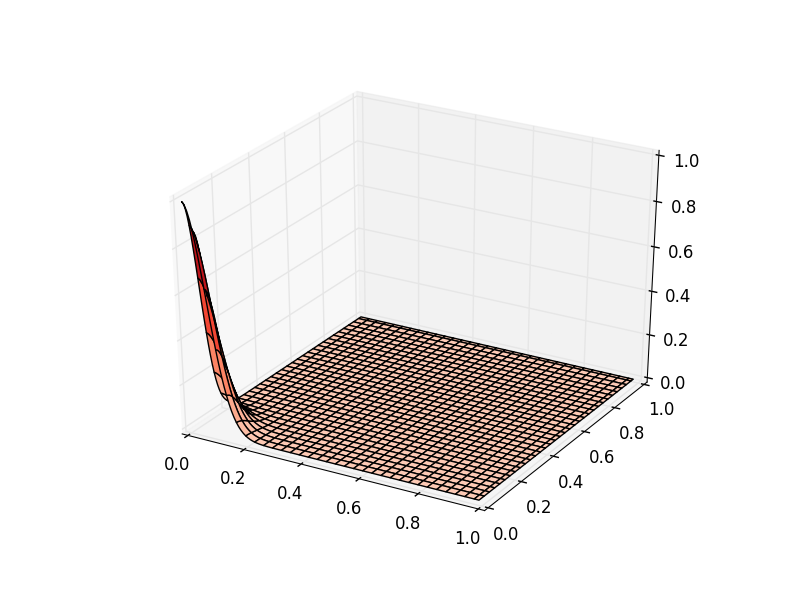
\includegraphics[scale=0.4]{partb_fig_frames/partb_fig01.png}%
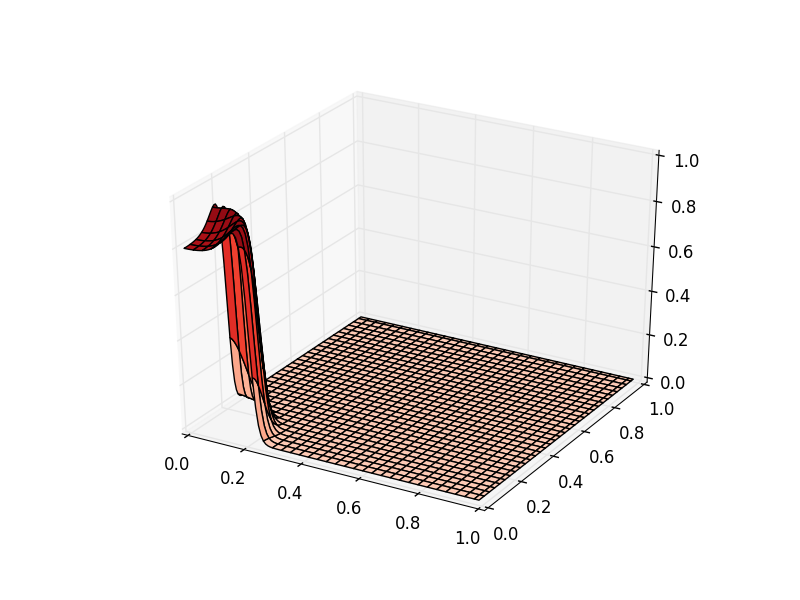
\includegraphics[scale=0.4]{partb_fig_frames/partb_fig03.png}
\caption{$t=0$ and $t=60$.}
\end{figure}
\begin{figure}[H]
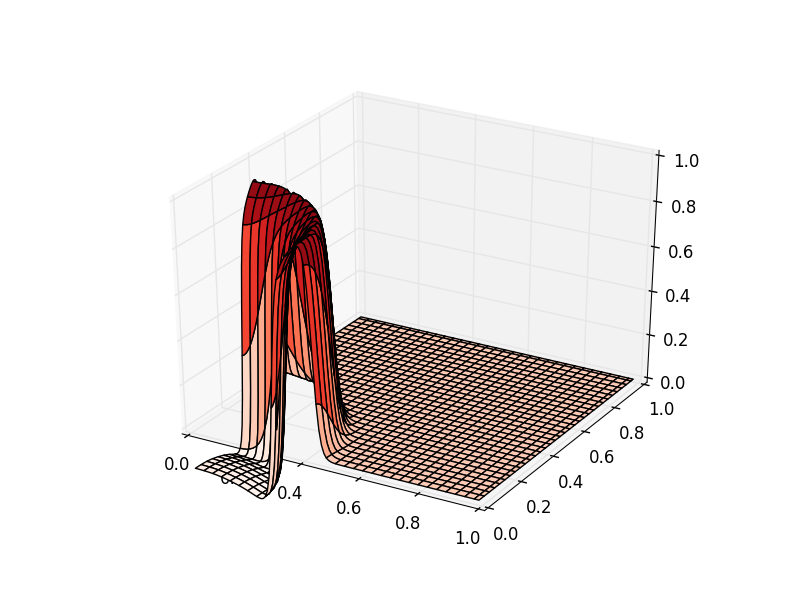
\includegraphics[scale=0.4]{partb_fig_frames/partb_fig05.png}%
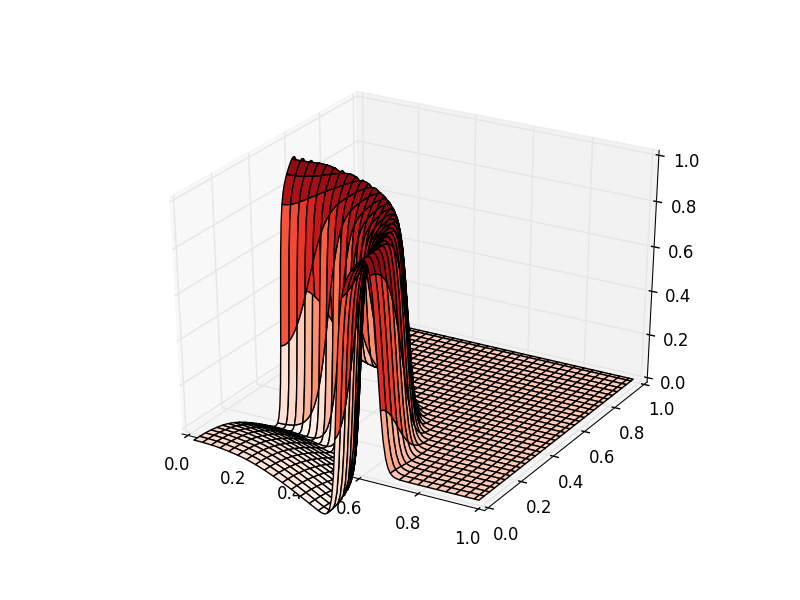
\includegraphics[scale=0.4]{partb_fig_frames/partb_fig07.png}
\caption{$t=120$ and $t=180$.}
\end{figure}
\begin{figure}[H]
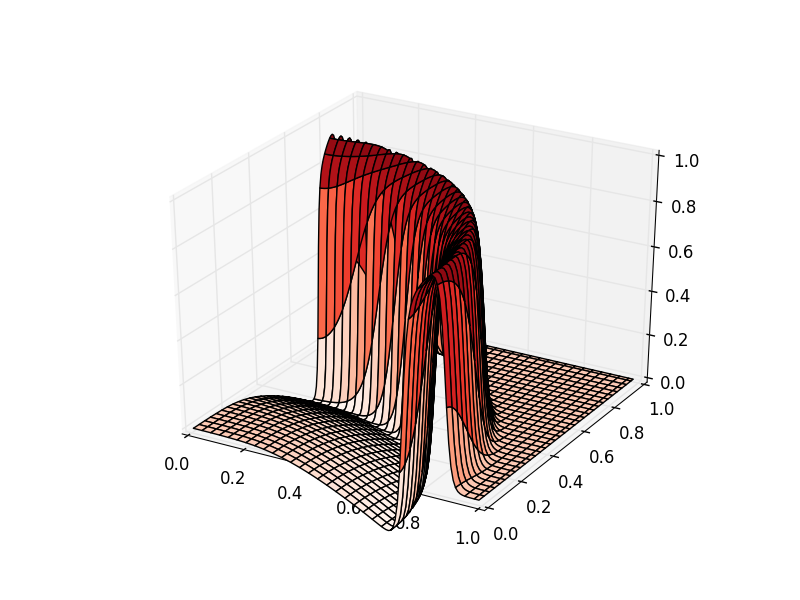
\includegraphics[scale=0.4]{partb_fig_frames/partb_fig09.png}%
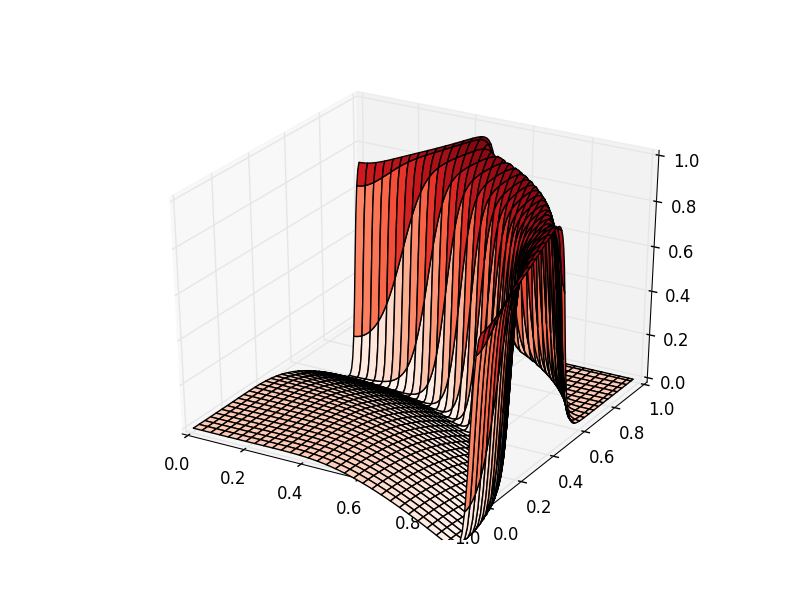
\includegraphics[scale=0.4]{partb_fig_frames/partb_fig11.png}
\caption{$t=240$ and $t=300$.}
\end{figure}

\item  Use the same parameters from part (b), but use the initial conditions
$$v(x,y,0) = 1-2x$$
$$w(x,y,0) = 0.05y$$
and run the simulation until time t = 600. Show the voltage at several points in time (pseudocolor plot, or contour plot, or surface plot $z = V (x, y, t)$) and describe the solution.
\end{enumerate}

The voltage solution in this case exhibits a spiral wave pattern throughout the grid that doesn't dampen out.  The spiral wave pattern forms since the nonhomogeneous recovery variable initial condition creates an imbalance in excitable and refractory neurons on the grid.  This allows the voltage spike to spread in one direction and not the other, which then loops back around when the refractory neurons become excitable again, and so on.

\begin{figure}[H]
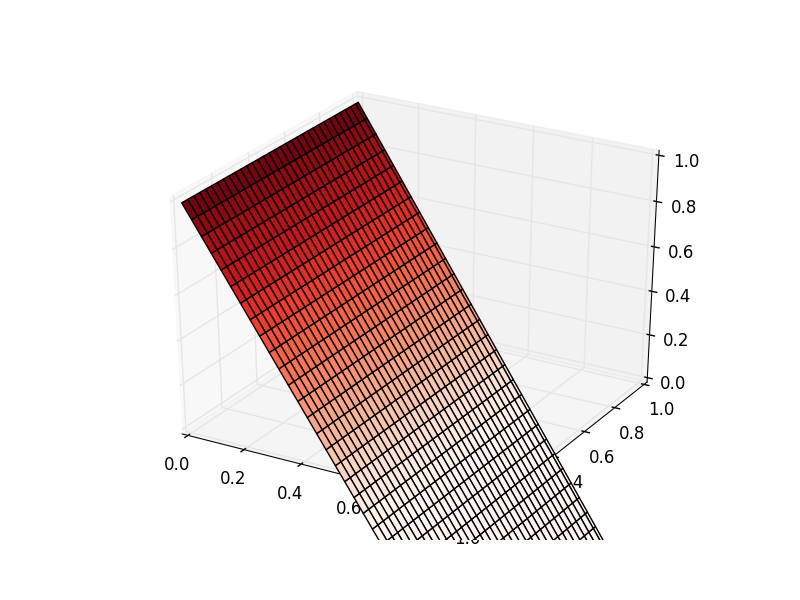
\includegraphics[scale=0.4]{partc_fig_frames/partc_fig01.png}%
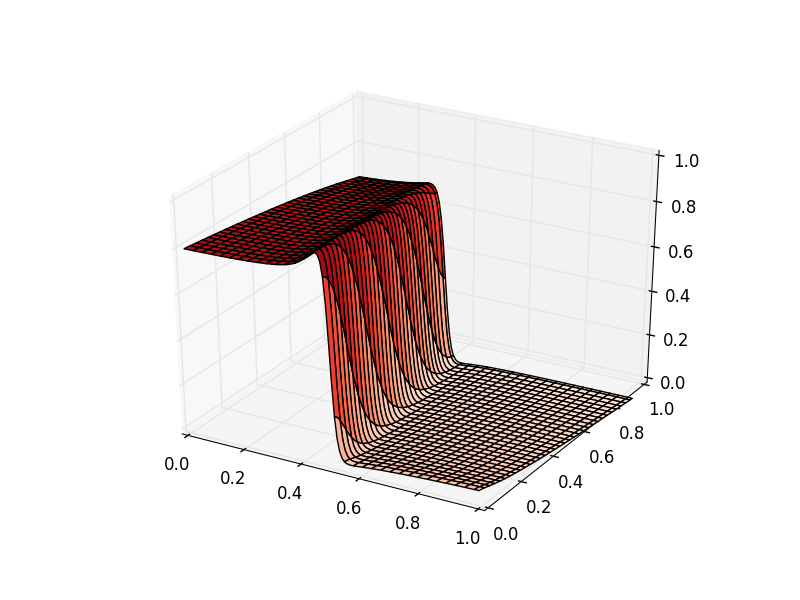
\includegraphics[scale=0.4]{partc_fig_frames/partc_fig03.png}
\caption{$t=0$ and $t=60$.}
\end{figure}
\begin{figure}[H]
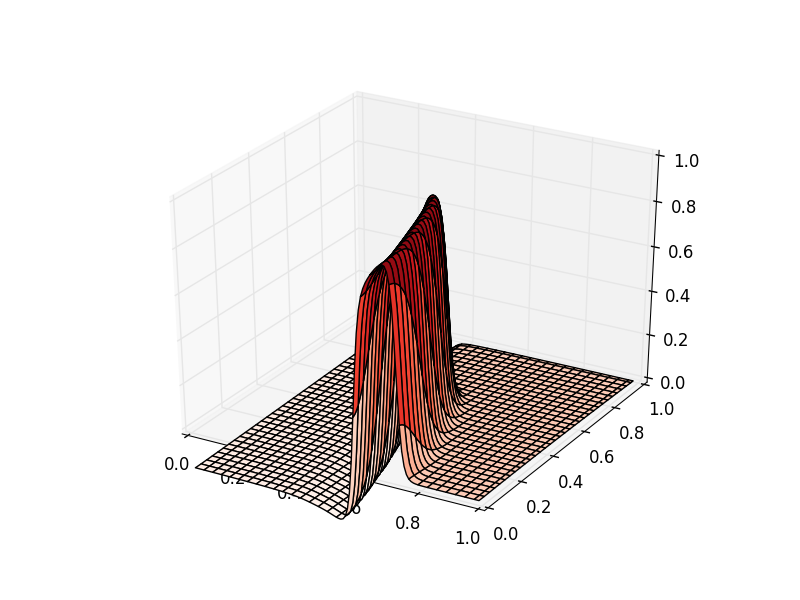
\includegraphics[scale=0.4]{partc_fig_frames/partc_fig05.png}%
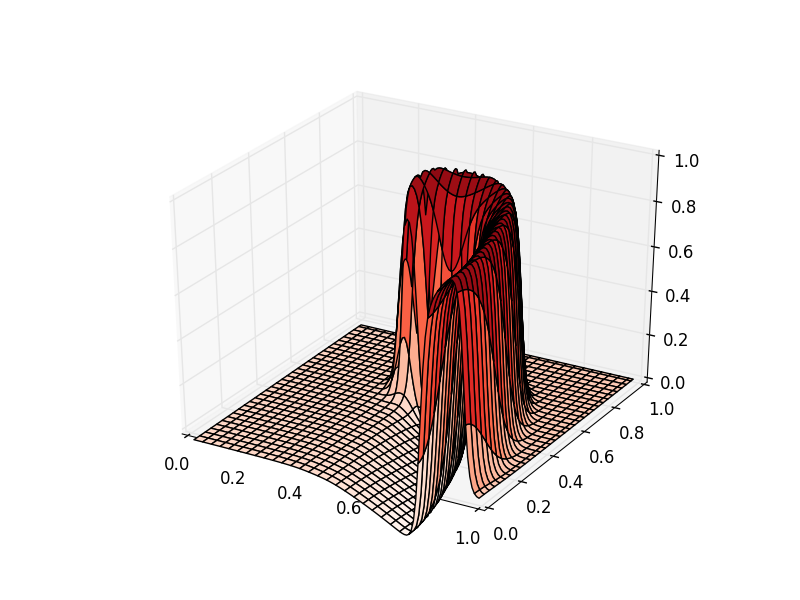
\includegraphics[scale=0.4]{partc_fig_frames/partc_fig07.png}
\caption{$t=120$ and $t=180$.}
\end{figure}
\begin{figure}[H]
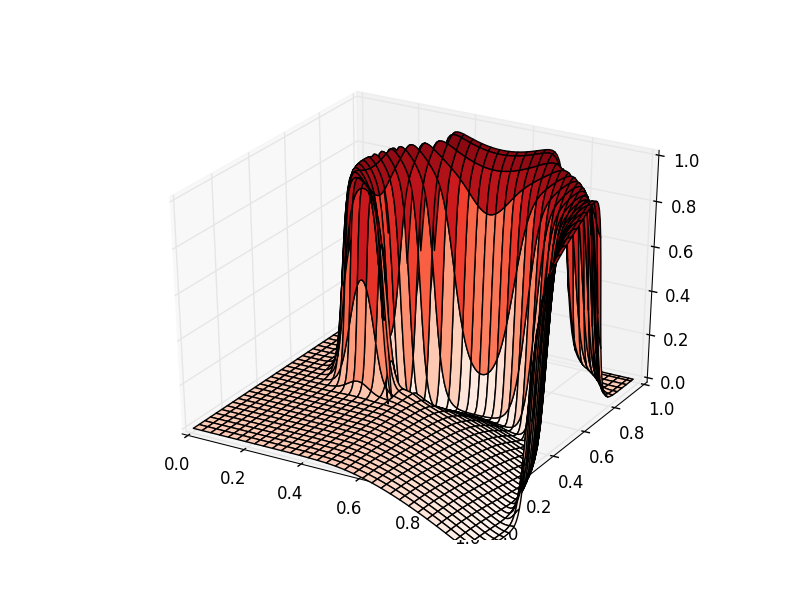
\includegraphics[scale=0.4]{partc_fig_frames/partc_fig09.png}%
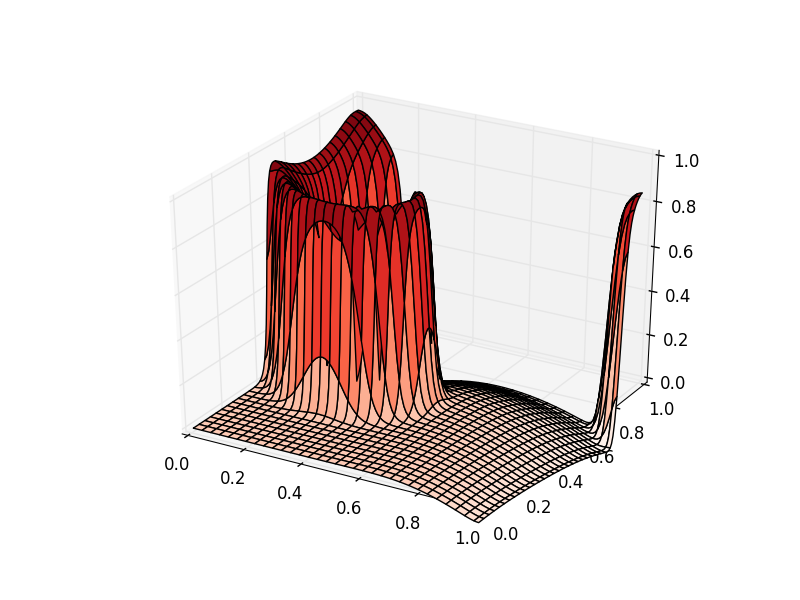
\includegraphics[scale=0.4]{partc_fig_frames/partc_fig11.png}
\caption{$t=240$ and $t=300$.}
\end{figure}
\begin{figure}[H]
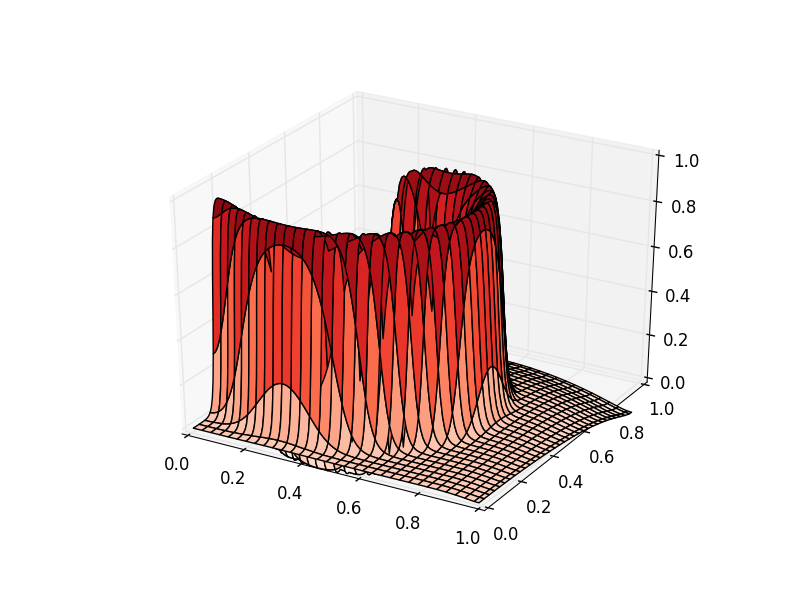
\includegraphics[scale=0.4]{partc_fig_frames/partc_fig13.png}%
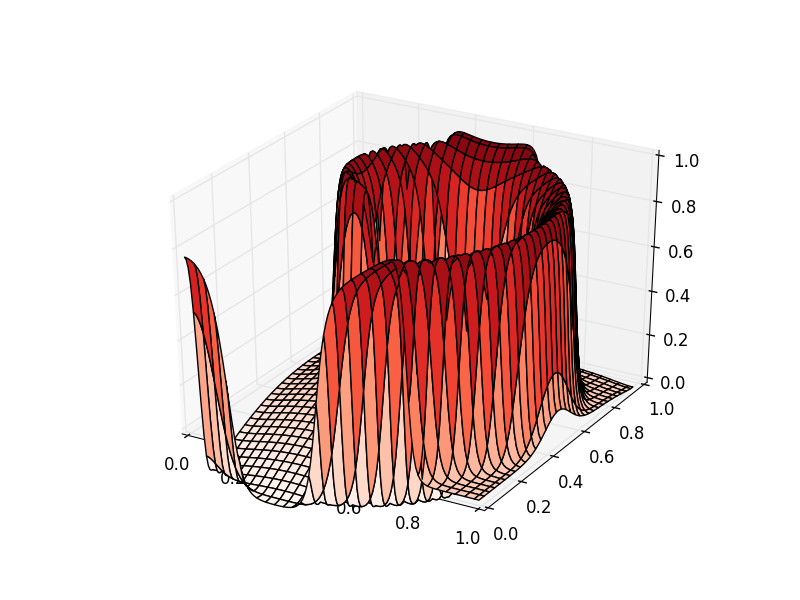
\includegraphics[scale=0.4]{partc_fig_frames/partc_fig15.png}
\caption{$t=360$ and $t=420$.}
\end{figure}
\begin{figure}[H]
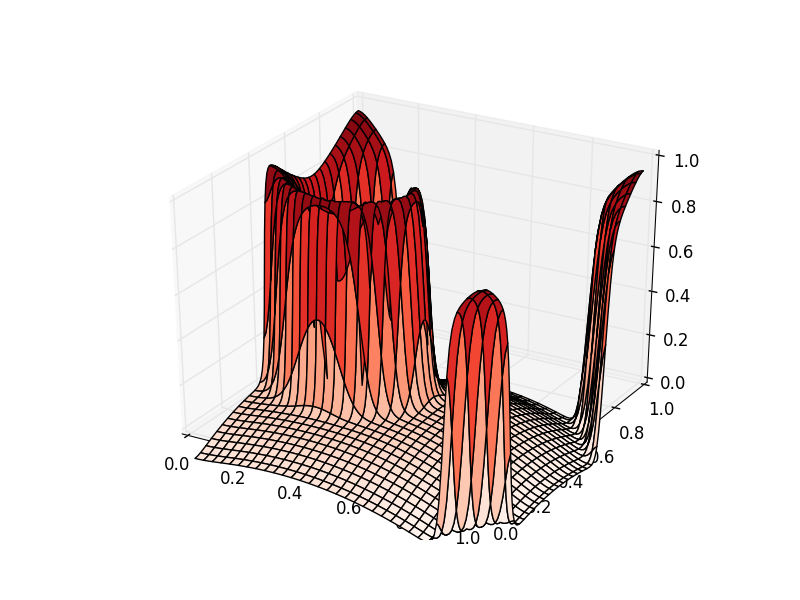
\includegraphics[scale=0.4]{partc_fig_frames/partc_fig17.png}%
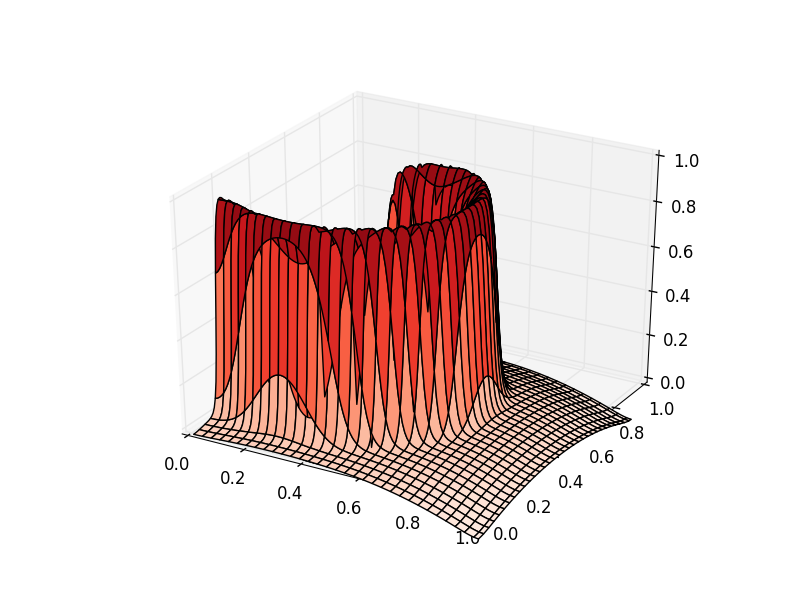
\includegraphics[scale=0.4]{partc_fig_frames/partc_fig19.png}
\caption{$t=480$ and $t=540$.}
\end{figure}
\begin{figure}[H]
\centering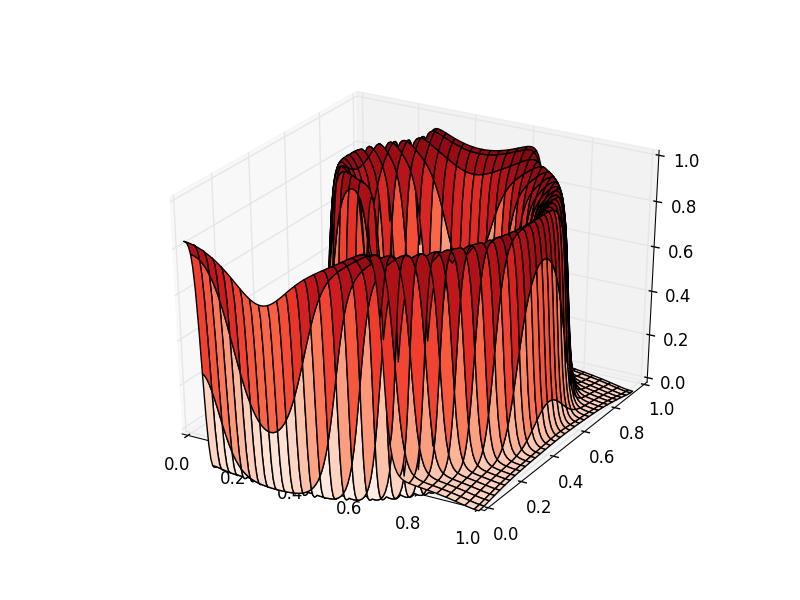
\includegraphics[scale=0.4]{partc_fig_frames/partc_fig21.png}
\caption{$t=600$.}
\end{figure}

%-------------------------------------------------------------------------------
\section*{Python Code}
The following code was used to generate the refinement study tables for problem 1:
\begin{verbatim}
#Problem1.py
#Carter Johnson
#Mat228B Assignment 3

#Refinement study on the
#Peaceman-Rachford ADI scheme on a cell-centered grid
#for solving 2-d homogeneous diffusion eqn with Neumann BCs

from __future__ import division

import numpy as np
import matplotlib.pyplot as plt
from mpl_toolkits.mplot3d import Axes3D
from numpy import exp
from numpy.linalg import norm
from tabulate import tabulate
from tqdm import tqdm
from time import clock
import scipy.sparse as sparse
import scipy.sparse.linalg

from peaceman_rachford import peaceman_rachford_method

def refinement_study():
    #refinement study for 2d diffusion using peaceman-rachford ADI scheme
    #for homogenous diffusion w/ Neumann bcs

    #set vector of grid spacings/time steps
    h = [2**(-i) for i in range(1,11)]

    #diffusion coefficient
    b = 0.1

    #Don't plot
    plotting=0

    #record successive differences + ratios, run times and runtime ratios
    diffs = np.zeros(len(h))
    diff_ratios = np.zeros(len(h))
    times = np.zeros(len(h))
    time_ratios = np.zeros(len(h))

    
    for i in tqdm(range(len(h))):
        #get time step
        delT = h[i]

        #get grid points for level h
        N = int(1/h[i])
        Nt = int(1/delT)
        X = [h[i]*(j-0.5) for j in range(1,N+1)]
        Y = [h[i]*(j-0.5) for j in range(1, N+1)]

        #initial condition u(x,y,0)=exp(-100((x-0.3)^2+(y-0.4)^2))
        u = [[exp(-100*((x-0.3)**2+(y-0.4)**2)) for x in X] for y in Y]
        u = np.asarray(u)


        toc=clock()
        u_new = peaceman_rachford_method(h[i], delT, b, u, plotting)
        tic=clock()
        if i>0:
            diffs[i]=(h[i-1]**2)*norm(restriction(u_new, h[i]) - u_old,ord=1)
            time_ratios[i] = (tic-toc)/times[i-1]
        if i>1:
            diff_ratios[i]=diffs[i-1]/diffs[i]
        u_old = u_new+0 
        times[i]=tic-toc


    table = [[h[i], times[i], time_ratios[i], diffs[i], diff_ratios[i]] for i in range(len(h))]
    print(tabulate(table, headers=["grid spacings/time steps", "Runtimes", "Runtime Ratios", "Successive Differences", "Difference Ratios"], tablefmt="latex"))

def restriction(u, h):
    u_f = u +0
    h2 = 2*h
    n2 = int(1/h2)
    u_c = np.zeros((n2, n2), dtype=float)

    #loop over coarse mesh
    for i in range(0,n2):
        for j in range(0,n2):
            u_c[i][j] = u_f[2*i+1][2*j+1]
    return u_c

if __name__ == '__main__':
    refinement_study()  
\end{verbatim}

The following code was used to implement the Peaceman-Rachford ADI scheme for both problems 1 and 2:
\begin{verbatim}
#Peaceman_Rachford.py
#Carter Johnson
#Mat228B Assignment 3

#Peaceman-Rachford ADI scheme on a cell-centered grid
#for solving 2-d homogeneous diffusion eqn with Neumann BCs

from __future__ import division

import numpy as np
import matplotlib.pyplot as plt
from mpl_toolkits.mplot3d import Axes3D
from numpy import exp
from numpy.linalg import norm
import scipy.sparse as sparse
import scipy.sparse.linalg

def sparse_matrices(h):
    #set sparse matrix L, the discrete 1-D Laplacian
    #for 3-pt centered flux 2nd order approximation
    #includes Neumann BCs

    #Set number of grid points
    N = int(1/h)

    #set off-diagonal Laplacian components
    off_diag = 1*np.ones(N)
    #set diagonal Laplacian components
    diag = (-2)*np.ones(N)
    diag[0] = -1
    diag[-1] = -1

    # Generate the diagonal and off-diagonal matrices
    A = np.vstack((off_diag, diag, off_diag))/(h**2)
    L = scipy.sparse.dia_matrix((A,[-1,0,1]),shape=(N,N))
    I = scipy.sparse.identity(N)

    return L, I

def peaceman_rachford_step(u,h,delT,b,L,I):
    N = int(1/h)
    #Diffuse in x direction
    # iterate over columns of u^n to get columns of u^*
    A = (I + (b*delT/2) * L)
    RHS_terms = A.dot(u)
    LHS_matrix = scipy.sparse.csc_matrix(I-(b*delT/2)*L)
    u_star = scipy.sparse.linalg.spsolve(LHS_matrix, RHS_terms) 

    #Diffuse in y direction
    #iterate over rows of u^* to get rows of u^n+1
    A = (I + (b*delT/2) * L)
    RHS_terms = A.dot(np.transpose(u_star))
    LHS_matrix = scipy.sparse.csc_matrix(I-(b*delT/2)*L)
    u_next = np.transpose(scipy.sparse.linalg.spsolve(LHS_matrix, RHS_terms))

    return u_next

def peaceman_rachford_method(h,delT,b,u_old, plotting):
    N = int(1/h)
    Nt = int(1/delT)

    #get operators
    [L, I] = sparse_matrices(h)

    energy = np.sum(u_old)
    
    if plotting==1:
        fig = plt.figure()
        ax = fig.add_subplot(111, projection='3d')
        # `plot_surface` expects `x` and `y` data to be 2D
        grid_X = [h*(i-0.5) for i in range(1,N+1)]
        grid_Y = [h*(j-0.5) for j in range(1, N+1)]
        X, Y = np.meshgrid(grid_X, grid_Y)  
        #keep z limits fixed
        ax.set_zlim(0, 1)
        plt.ion()
        #plot first frame, u(x,y,0)
        frame = ax.plot_surface(X, Y, u_old)
        plt.pause(0.05)


    for t in range(Nt):
        #solve for next u
        u_new = peaceman_rachford_step(u_old, h, delT, b, L, I)
        
        if plotting==1:
            #plot current u
            ax.collections.remove(frame)
            frame = ax.plot_surface(X, Y, u_new)
            plt.pause(0.05)

        u_old = u_new + 0
        energy2 = np.sum(u_new)
        # print(energy-energy2)


    energy2 = np.sum(u_new)
    print(energy-energy2)
    return u_new
\end{verbatim}

The following code was used to generate the solutions to the FitzHugh Nagumo equation and voltage plots for problem 2:
\begin{verbatim}
#Fractional_Step_Reaction_Diffusion.py
#Carter Johnson
#Mat228B Assignment 3

#Fraction Step Strang-splitting method to solve Fitzhugh-Nagumo 
#Reaction-diffusion eqn
#using Peaceman-Rachford ADI scheme on a cell-centered unit square grid
#for solving 2-d homogeneous diffusion part with Neumann BCs
#and runge-kutta 2 for reaction term ode 

from __future__ import division

import numpy as np
import matplotlib.pyplot as plt
from matplotlib import cm
from mpl_toolkits.mplot3d import Axes3D
from numpy import exp
from numpy.linalg import norm
from tqdm import tqdm
from pylab import savefig
import scipy.sparse as sparse
import scipy.sparse.linalg
from scipy.integrate import ode
from peaceman_rachford import peaceman_rachford_method, peaceman_rachford_step, sparse_matrices

def f(u,a=0.1,I=0,eps=0.005,gamma=2):
    #Reaction terms for Fitzhugh-Negumo model
    return np.c_[(a-u[:,0])*(u[:,0]-1)*u[:,0]-u[:,1]+I, eps*(u[:,0]-gamma*u[:,1])]

def rk2(u,delT):
    #Runge-Kutta 2 Method - simple 2nd order explicit ODE solver
    u_star = u + delT/2*f(u)
    return u+delT*f(u_star)

def strang_split_step(v,w, h, delT, b, L, I):
    #Strang splitting time step for fractional step method solve
    # v = bLv + R(v,w)
    # w = R(v,w)
    N = int(1/h)

    #first solve diffusion on v using ADI scheme for time length delt/2
    v_star = peaceman_rachford_step(v,h,delT/2,b,L,I)

    #then solve reaction for delt using a ODE solver
    #flatten v and w from grid-lined up matrices into column vectors, put side by side
    v_and_w = np.c_[v_star.flatten(), w.flatten()]
    #solve ODE at each grid point (row of v_and_w) for one time step delt
    v_w_star = rk2(v_and_w,delT)
    #reshape back into v, w grid matrices
    v_starstar = np.reshape(v_w_star[:,0], (N,N))
    w_next = np.reshape(v_w_star[:,1], (N,N))

    #solve diffusion on v_starstar for delt/2 to get v_next
    v_next = peaceman_rachford_step(v_starstar,h,delT/2,b,L,I)

    return v_next, w_next
    

def frac_step_strang_split(h, delT, Nt, b, v_old, w_old, plotting):
    #Strang splitting fractional step method
    #solve reaction-diffusion eqn for v,w
    #up to time Nt
    N = int(1/h)

    #get operators
    [L,I] = sparse_matrices(h)

    #set oldest v,w for ab2 solver
    old_vw = np.c_[v_old.flatten(), w_old.flatten()]

    #set up plotting
    if plotting[0]==1:
        fig = plt.figure()
        ax = fig.add_subplot(111, projection='3d')
        # `plot_surface` expects `x` and `y` data to be 2D
        grid_X = [h*(i-0.5) for i in range(1,N+1)]
        grid_Y = [h*(j-0.5) for j in range(1, N+1)]
        X, Y = np.meshgrid(grid_X, grid_Y)  
        #keep z limits fixed
        ax.set_zlim(0, 1)
        plt.ion()
        #set colors for plot
        my_col = cm.Reds
        #plot first frame, v(x,y,0)
        frame = ax.plot_surface(X, Y, v_old, cmap=my_col, vmin=-0.25, vmax=1, rstride=4, cstride=4)
        plt.pause(0.05)
        #save first frame
        # frame_no=1
        # filename=plotting[2]+'_fig0'+str(frame_no)+'.png'
        # savefig(filename)

    #run simulation for Nt time steps
    for t in tqdm(range(Nt)):
        #solve for next v and w
        [v_new,w_new] = strang_split_step(v_old,w_old, h, delT, b, L, I)
        
        if plotting[0]==1 and t%plotting[1]==0:
            #plot current v
            ax.collections.remove(frame)
            frame = ax.plot_surface(X, Y, v_new, cmap=my_col,vmin=-0.25, vmax=1, rstride=4, cstride=4)
            # ax.view_init(30,t/20)
            plt.pause(0.001)
            # if t%(5*plotting[1])==0:
            #   frame_no=frame_no+1
            #   if frame_no<10:
            #       filename=plotting[2]+'_fig0'+str(frame_no)+'.png'
            #   else:
            #       filename=plotting[2]+'_fig'+str(frame_no)+'.png'
            #   savefig(filename)


        v_old = v_new + 0
        w_old = w_new


    return v_new, w_new

def part_b_Run(h,delT,plotting):
    #parameters
    N = int(1/h)
    Nt = 300*int(1/delT)
    a = 0.1
    gamma = 2
    eps = 0.005
    I_current=0
    D = 5*(10**(-5))

    #setup initial data
    grid_X = [h*(i-0.5) for i in range(1,N+1)]
    grid_Y = [h*(j-0.5) for j in range(1, N+1)]
    v0 = np.asarray([[exp(-100*(x**2+y**2)) for x in grid_X] for y in grid_Y])
    w0 = np.asarray([[0*x+0*y for x in grid_X] for y in grid_Y])
    
    #run Fractional Step method to solve up to time Nt
    [v,w] = frac_step_strang_split(h,delT,Nt,D, v0,w0, plotting)

def part_c_Run(h,delT,plotting):
    #parameters
    N = int(1/h)
    Nt = 1000*int(1/delT)
    a = 0.1
    gamma = 2
    eps = 0.005
    I_current=0.0
    D = 5*10**(-5)

    #setup initial data
    grid_X = [h*(i-0.5) for i in range(1,N+1)]
    grid_Y = [h*(j-0.5) for j in range(1, N+1)]
    v0 = np.asarray([[1-2*x for x in grid_X] for y in grid_Y])
    w0 = np.asarray([[0.05*y for x in grid_X] for y in grid_Y])
    
    #run Fractional Step method to solve up to time Nt
    [v,w] = frac_step_strang_split(h,delT,Nt,D, v0,w0, plotting)

if __name__ == '__main__':
    h = 2**(-7)
    delT = 2**(-5)
    frames=100
    plot_on=1
    part_b_Run(h,delT,[plot_on,frames,'partb'])
    part_c_Run(h,delT,[plot_on, frames, 'partc_spin'])  
\end{verbatim}
\end{document}